\subsubsection{Schwungräder}
\begin{wrapfigure}{r}{0.50\textwidth}
	\centering
	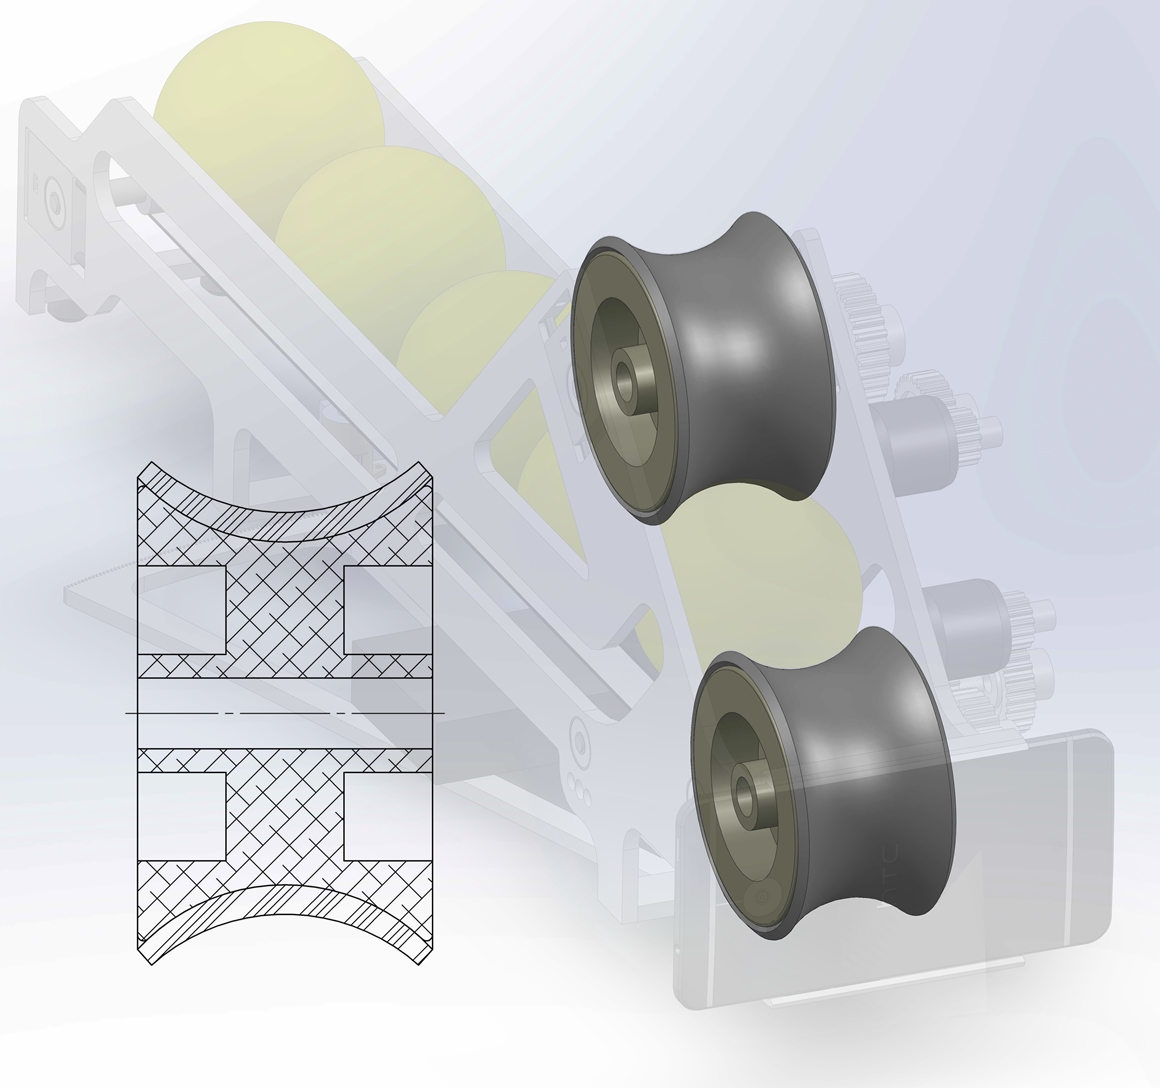
\includegraphics[width=0.5\textwidth]{Enddokumentation/Loesungskonzept/Bilder/Schwungraeder.jpg}
	\caption{Schwungräder}
	\label{fig:Schwungräder}	
\end{wrapfigure}
Die Vortriebskraft für die Tennisbälle wird durch zwei Schwungräder übertragen. Der
Schwungradantrieb wurde aus mehreren Gründen gewählt. Über die Drehzahl, Kraft der Motoren oder
durch Übersetzungen lässt sich die Geschwindigkeit der Bälle nahezu stufenlos einstellen. Man kann
durch vorhergehende Berechnungen die ungefähren Grössen, Leistungen und Kräfte eruieren und das
System so auslegen, dass später nur noch Parameter geändert werden müssen ohne kostspielige Bauteile
anzupassen oder gar zu ersetzten. Weiter ist durch die konkave Form der Schwungräder die Richtung der 
Ballflugbahn vorgegeben. Hier wird keine zusätzliche Ballführung gebraucht was Gewicht, Kosten und
Platz spart. Die Räder sind konkav ausgearbeitet, so dass die Beschleunigung nicht nur über einen
Punkt übertragen wird. So wird gewährleistet, dass die Kraft über eine grössere Fläche
übertragen werden kann. Dadurch entsteht der Vorteil, dass die Beschleunigung geführt
abläuft, wodurch ein gerichteter Wurf entsteht. So kann die vorhandene Rotationsenergie vollumfänglich 
den Tennisbällen übergeben werden. Die Ausrundung wird durch den Radius der Bälle
gegeben. Der Durchmesser der Schwungräder ist so festgelegt, dass mit der vorhandenen Masse ein
genügendes Trägheitsmoment zur Verfügung steht. Dies ist nötig, damit bei der Beschleunigung der
Tennisbälle die Schwungräder nicht zu stark abgebremst werden. Dennoch sollten sie nicht zu schwer
oder zu gross sein, da das Gewicht einer der Faktoren in der Gesamtbewertung ist. Die Grösse beruht
deshalb auf einem Kompromiss. Durch den Durchmesser wird auch die Winkelgeschwindigkeit
festgelegt. Die Schwungräder sind aus PVC\footnote{\textbf{P}oly\textbf{V}inyl \textbf{C}hlorid}
gefertigt. Dieser Werkstoff ist einfach zu bearbeiten und bietet zugleich eine genügend grosse
Festigkeit. Die Räder sind mit einer speziellen Haftmatte beschichtet, damit die Kraft optimal auf
den Ball übertragen werden kann. Somit wird ein höherer Haftreibungskoeffizient erreicht, der ein
Durchrutschen der Bälle verhindert. Die Schwungräder besitzen grosses Optimierungspotential,
da die vorhandene Rotationsenergie der entscheidende Faktor ist. Die Achsen der zwei Schwungräder
sind im Winkel von 45$^\circ$ zur Bodenplatte angeordnet. Der Abschusswinkel ist so gewählt, dass die
Tennisbälle in einem genug grossen Einschlagwinkel im Zielbereich landen und keine Möglichkeit
besteht mit dem Korbrand zu kollidieren. Das Verhältnis von Wurfkraft zu Wurflänge ist beim Winkel
von 45$^\circ$ auch am besten. Die Wurfweite wird durch die Drehzahl der Schwungräder gesteuert. Der
Achsenabstand der beiden Räder bestimmt die Presskraft der einzelnen Bälle. Dies wiederum trägt zur
Abbremsung der Schwungräder bei, welche nicht zu gross sein darf, damit die einzelnen Bälle in
kurzem Abstand hintereinander zugeführt werden können. Die konkave Form der Räder gibt dem Ball die
genaue Richtung der Flugbahn vor.
	
	
	